\documentclass[11pt]{article} % use larger type; default would be 10pt
\usepackage[utf8]{inputenc} % set input encoding (not needed with XeLaTeX)
\usepackage[T1]{fontenc}
\usepackage{authblk}

%%% BEGIN Article customizations

%%% PAGE LAYOUT
\usepackage{geometry} % to change the page dimensions
\geometry{a4paper} % or letterpaper (US) or a5paper or....
% \geometry{margin=1in} % for example, change the margins to 2 inches all round
\usepackage[parfill]{parskip} % Activate to begin paragraphs with an empty line rather than an indent

%%% FIGURES
\usepackage{graphicx} % support the \includegraphics command and options
\graphicspath{{../FIGURES/FIGURE_PDFS/}}

%%% PACKAGES
\usepackage{booktabs} % for much better looking tables
\usepackage{array} % for better arrays (eg matrices) in maths
\usepackage{paralist} % very flexible & customisable lists (eg. enumerate/itemize, etc.)
\usepackage{verbatim} % adds environment for commenting out blocks of text & for better verbatim
\usepackage{subfig} % make it possible to include more than one captioned figure/table in a single float
\usepackage{lscape}
\usepackage{amsmath}
\usepackage{amssymb}
\usepackage{color}
% These packages are all incorporated in the memoir class to one degree or another...

%%% HEADERS & FOOTERS
\usepackage{fancyhdr} % This should be set AFTER setting up the page geometry
\pagestyle{fancy} % options: empty , plain , fancy
\renewcommand{\headrulewidth}{0pt} % customize the layout...
\lhead{}\chead{}\rhead{}
\lfoot{}\cfoot{\thepage}\rfoot{}

%%% SECTION TITLE APPEARANCE
\usepackage{sectsty}
\allsectionsfont{\sffamily\mdseries\upshape} % (See the fntguide.pdf for font help)
% (This matches ConTeXt defaults)

%%% ToC (table of contents) APPEARANCE
\usepackage[nottoc,notlof,notlot]{tocbibind} % Put the bibliography in the ToC
\usepackage[titles,subfigure]{tocloft} % Alter the style of the Table of Contents
\renewcommand{\cftsecfont}{\rmfamily\mdseries\upshape}
\renewcommand{\cftsecpagefont}{\rmfamily\mdseries\upshape} % No bold!

%%%Bibliography
\usepackage{natbib}
\usepackage{url}

%%% END Article customizations

%%% Title and author are here
\title{Reproducibility of SNV-calling in multiple sequencing runs from single tumors}
\author[1]{Dakota Z. Derryberry\thanks{dakotaz@utexas.edu}}
\author[2,3]{Matthew C. Cowperthwaite}
\author[1,4]{Claus O. Wilke} 
\affil[1]{The University of Texas at Austin, Cell \& Molecular Biology}
\affil[2]{St. David's NeuroTexas Institute Research Foundation}
\affil[3]{Center for Systems and Synthetic Biology, The University of Texas at Austin}
\affil[4]{The University of Texas at Austin, Integrative Biology}

\begin{document}
\maketitle

\section*{Abstract}

We examined 55 technical sequencing replicates of Glioblastoma multiforme (GBM) tumors from The Cancer Genome Atlas (TCGA) to ascertain the degree of repeatability in calling single-nucleotide variants (SNVs). We used the same mutation-calling pipeline on all pairs of samples, and we measured the extent of the overlap between two replicates, that is, how many specific point mutations were found in both replicates. We further tested whether additional filtering increased or decreased the size of the overlap.  We found that about half of the putative mutations identified in one sequencing run of a given sample were also identified in the second, and that this percentage remained steady throughout orders of magnitude of variation in the total number of mutations identified (from 23 to 10,966). We further found that using filtering after SNV-calling removed the overlap completely. We concluded that there is variation in the frequency of mutations in GBMs, and that while some filtering approaches preferentially removed putative mutations found in only one replicate, others removed a large fraction of putative mutations found in both.

\section*{Introduction}

The past six years have seen an explosion of data in cancer genomics, an effort led by TCGA, an archive of publicly-available data that includes sequencing of paired tumor-normal samples from individual patients for thousands of tumors \citep{TCGA-GBM, TCGA-GBM-13}. TCGA's database includes hundreds of samples of each of several tumor types, including over 500 samples of Glioblastoma multiforme (GBM), the most common and deadly primary brain tumor. GBM has a median survival time of 14 months and a 5-year survival rate of ~5\%. Prognosis for patients with this disease remains poor despite significant research investment, due to the difficulty of surgical resection and the limited number of effective chemotherapeutics \citep{GBM-stats}. To work towards the goal of improving patient outcomes using precision medicine, TCGA and other groups \citep{Parsons} used large-scale genomics data to discover genes and pathways mutated in GBM \citep{pathways}, discover different GBM subtypes \citep{subtypes}, and develop a variety of computational models to find GBM driver mutations \citep{drivers}.

However, these and other efforts have produced very few results for patients in terms of improved treatments. It may be that we simply haven't yet analyzed the data in the most informative manner. Another factor may be that the data are noisy. It is well known that sequencing and variant-calling pipelines are not error-free. For example, different pipelines for calling single-nucleotide variants (SNVs) can return different results on the same data \citep{SNPcall}. Given the heterogeneity in cancer genomes \citep{heterogenous1, heterogenous2}, and the presence of functional low-frequency variants in GBM \citep{rare}, the signal-to-noise ratio in the TCGA dataset may be particularly low. Yet despite widespread use of this dataset, and significant monetary investment in collecting and analyzing the data, we know little about how to maximize the quality of the sequence data and SNV-calls. One way to address this question would be to analyze technical replicates of sequencing data \citep{replicates}. Here, we addressed one aspect of this question, by asking whether the same SNV-calling pipeline will return comparable results on two sequencing runs from the same tissue. And further, we asked whether added filtering after SNV-calling increases or decreases the degree of similarity among replicates.

We answered these questions using TCGA data from 55 GBM tumors that were sequenced twice, once each with (i) the standard whole-genome sequencing (WGS) protocol, and (ii) an additional amplification step before library prep, which we refer to as the whole-genome amplification (WGA) protocol. For each of these 55 technical replicate pairs, we compared the somatic variants found in the WGS and WGA replicates, before and after analyzing the variants using various SNV-filtering approaches. We found significant overlap (around 50\%) between technical replicates, but also significant differences. As expected, the additional amplification step in the WGA protocol versus the WGS protocol added some putative mutations to the sample, so that on average these replicates had (i) more putative mutations, and (ii) a smaller percentage overlap between replicates. We found that the number of mutations in the WGS replicates varied by orders of magnitude, from 110 to 8,192. Contrary to expectations, the percentage overlap between technical replicates did not decrease with increasing numbers of putative mutations, suggesting real variation in mutation frequency between samples. This result may be in part due to known mutational hotspots in some tumors \citep{Karen}. Our attempt to use SNV filtering, either via SomaticSniper \citep{SomaticSniper} or via custom-built filters, to increase the similarity between technical replicates was unsuccessful: Filtering removed almost the entirety of the overlap between the replicates.

\section*{Results}

\subsection*{How similar are two replicate sequencing runs of the same tumor?}

% Experiment: size of overlap (figures 3 and 4)
%(a) a brief (one sentence to one paragraph) summary of what you did and why
%(b) a description of what you found carrying out this experiment

DNA sequencing is not error-free. Error is introduced by mis-called bases in sequencing runs and by mis-aligned bases during sequence analysis \citep{seqerror}. Loss of heterozygosity may be a real feature of the data, or an amplification artifact that occurs when only one allele of a polymorphic site is amplified. Cancer DNA is highly heterogenous, which makes for an additional source of error: A mutation present in only some tumor cells may or may not be present in a given sample at high enough frequency to be seen, so that a polymorphic mutation may appear fixed or completely absent. In general, we would like to know how often these errors occur. One way of investigating this question would be to use an orthogonal technique such as PCR to verify each individual mutation. However, this method is expensive and time consuming. A cheaper alternative would be to sequence the tumor multiple times and to look at the similarity between replicates. Theoretically, any fixed mutation will appear in all replicates, while errors due to (i) sequencing errors, (ii) amplification errors, or (iii) alignment errors will not. (Polymorphic mutations would be present in some but not all samples, so this method does not address the difficulty of calling low-frequency variants in tumors.) The multiple-sequencing approach is used in most biological sequencing experiments, but not generally in cancer genomics, presumably due to unavailability of additional pathology specimens and the expense of sequencing multiple replicates for each of the hundreds of samples necessary for cancer genomics research. Nevertheless, even if researchers cannot verify every mutation or sequence multiple replicates for each tumor, it would be useful to know what percentage of called mutations would be likely to appear in additional sequencing replicates.

TCGA's GBM data set includes 2 technical replicates for each of 55 tumors. In this case, the technical replicates are not identical. One protocol included an additional amplification step \citep{TCGA-GBM}, and we refer to this replicate as the WGA (whole-genome amplification) replicate, and the other as the WGS (whole-genome sequencing) replicate. Despite the difference in sequencing protocol, we would expect any fixed mutation to appear in both replicates, while polymorphic mutations and sequencing error might appear in only one. Consequently, those putative mutations appearing in both replicates are more likely to be real somatic variants than those found in only one replicate. We further hypothesized that the WGA samples would have a greater number of amplification errors, and thus more putative SNVs per sample, than the corresponding WGS samples. 

For each patient (n=55), we called mutations in both technical replicates and in the patient's blood sample, using the same computational pipeline (see Figure~\ref{fig:pipeline} and Methods): We downloaded TCGA BAM files with CGHub \citep{CGHub}, re-generated fastq files with picard \citep{picard}, re-aligned the fastq files to hg19 with bwa \citep{bwa}, performed indel re-alignment and base recalibration with GATK \citep{GATK}, and finally called somatic mutations with SomaticSniper \citep{SomaticSniper}. We then compared the VCFs produced by SomaticSniper for each of the two technical replicates, and calculated the number of somatic mutations called in each replicate and the number of individual somatic mutations called in both replicates (hereafter, the overlap, see Figure~\ref{fig:pipeline}). We further calculated the percentage of mutations in each replicate that occurred in the overlap between the two. 

There were on average 844 putative mutations in the WGS replicates and 1,531 putative mutations in the WGA replicates (Table~\ref{tab:summary_stats}). Across all samples, the number of mutations in a given WGS replicate was correlated with the number of mutations in its corresponding WGA replicate (Pearson $r=0.51$, $df=53$, $P=8.35\times10^{-5}$, Figure~\ref{fig:C282_v_C484}). As expected, for each sample the WGA replicate (with the additional amplification step) had slightly more mutations overall, with a slightly smaller percentage appearing in the overlap (Figures~\ref{fig:C282_v_C484} and~\ref{fig:unfiltered_overlap}). We further found that the percent overlap between the two samples, calculated as $\text{WGA} \cap \text{WGS}/\text{WGS}$ for WGS replicates and $\text{WGA} \cap \text{WGS}/\text{WGA}$ for WGA replicates, was fairly consistent, on average 31\% in WGA replicates and 44\% in WGS replicates (Table~\ref{tab:summary_stats}). As expected, the distribution was narrower and taller in the WGS replicates, because on the whole the WGA samples had more amplification errors than the WGS samples (Figure~\ref{fig:unfiltered_overlap}).

% Experiment: number of mutations (figure 4)
%(a) a brief (one sentence to one paragraph) summary of what you did and why
%(b) a description of what you found carrying out this experiment
Although the percent overlap in WGS and WGA samples was fairly constant across samples, and the numbers of putative mutations in WGS and WGA samples were correlated, the exact number of putative mutations varied by orders of magnitude (Table~\ref{tab:summary_stats}). It is known that different cancers mutate at different rates: Some pediatric cancers have very few mutations \citep{RB2hit, pediatric}, while some adult tumors show a mutator phenotype leading to vastly increased numbers of mutations, usually resulting from errors in DNA repair pathways \citep{mutator}. GBM specifically is thought to have a relatively low mutation rate \citep{Parsons, TCGA-GBM-13}, and while some of our samples had low mutation frequencies in line with this theory (29 out of 110 samples had a mutation frequency within a factor of 2 of the reported 3 mutations per Mbp genome), several samples also had mutation frequencies an order of magnitude greater (24 out of 110 samples had a mutation frequency greater than 30 mutations per Mbp genome). One possible explanation is a degraded DNA sample or otherwise bad data. If this were the case, we would expect the percentage of the overlap between replicates (a measure of data quality) to decrease with the overall number of putative mutations. However, we found no significant correlation (Pearson $r=-0.04$, $df=53$, $P=0.76$) between the number of putative mutations in the WGS replicate and the percentage of those mutations that were in the overlap between replicates (Figure~\ref{fig:unfiltered_total_muts}). Thus, our data suggest that some samples may simply have a higher mutation frequency than others, or indeed than is generally supposed in GBM.

\subsection*{Does more sophisticated SNV filtering software increase or decrease the degree of similarity between replicates?}

% Experiment: which filters do what (figures 6 and 7) 
% Experiment: those two filters are different (figures 8 and 9)
%(a) a brief (one sentence to one paragraph) summary of what you did and why
%(b) a description of what you found carrying out this experiment
As an additional computational validation step for somatic mutations, it is common practice to employ computational algorithms that attempt to distinguish somatic mutations from germ line mutations and sequencing errors \citep{SomaticSniper, mut_calling}. Software platforms to perform these tasks are plentiful, and each one typically employs multiple methods to identify true positive mutations. The two platforms used in this research, SomaticSniper \citep{SomaticSniper} and GATK \citep{GATK}, calculate one or more quality scores based on features of the dataset and the individual reads, and putative mutations with higher quality scores are considered to be more likely true somatic mutations than those with low quality scores. In addition to considering these quality scores, there are additional filtering steps that one can use to distinguish true somatic mutations from errors of all sorts. Table~\ref{tab:filters} lists eight distinct SNV filters we evaluated. The first three are based on the quality scores generated by GATK and SomaticSniper.  We simply remove from the dataset anything that fails to meet conventional quality-score thresholds. The other five are additional filters that we developed for this project. Each of these five filters represents an aspect of the data or the putative mutation that is generally thought to indicate that a given SNV call is a false positive.

We first asked whether filtering the data increases or decreases the percentage of the sample that is overlapping between the two technical replicates. We expect that this analysis informs us about whether filtering out putative somatic mutations with these features affects the proportion of true somatic mutations in the remaining dataset. We found that, after removing putative mutations tagged by any one of the eight filters, the number of putative mutations per replicate decreased from 23--10,966 to 0--14 (Table~\ref{tab:summary_stats}). The size of the overlap between technical replicates decreased to 0--2 per sample, with 0 as the mode, i.e., the overall overlap percentage also decreased. We concluded that running all the filters on the data, in the absence of any other verification method, was counterproductive, because it removed all of the signal (as well as all the noise). 

We next looked at the individual effects of six of the eight filters. (We did not specifically study the GATK and SS filters, since both are directly linked to read quality.) We first considered the total number of putative SNVs removed by each filter (Figure~\ref{fig:boxplot_number_filtered}). We found that different filters removed different numbers of mutations, and that the lion's share of mutations were removed by the VAQ (Variant Allele Quality) and LOH (Loss of Heterozygosity) filters, which removed on average 309 and 539 putative SNVs, respectively (Table~\ref{tab:summary_stats}). Three other filters, those removing overlap with dbSNP and mutations within a 10 bp window of indels or other SNVs, removed 16, 28, and 46 putative mutations per sample, respectively (Figure~\ref{fig:boxplot_number_filtered} and Table~\ref{tab:summary_stats}). The final filter, which removed putative SNVs with less than 10\% coverage of the alternate allele, removed 1 putative SNV on average. 

We next asked how many of the SNVs removed by each filter were SNVs present in the overlap between technical replicates, and how many were in just one sample? Put differently, what percentage of putative SNVs removed by a given filter was in the category more likely to be true positives (overlap), versus the category more likely to be false positives (only present in one replicate)? To answer this question, we plotted the percent of the overlap (per sample) that was removed by each of the six filters (Figure~\ref{fig:boxplot_percent_overlap_filtered}). We found that the three filters removing overlap with dbSNP and putative mutations within 10bp of an indel or another SNV removed, on average, only 3\%--4\% of the overlap (Table~\ref{tab:summary_stats}). By contrast, the VAQ filter (specific to SomaticSniper) and the LOH filter each removed 53\% and 51\% of the overlap, respectively (Figure~\ref{fig:boxplot_percent_overlap_filtered}, Table~\ref{tab:summary_stats}). Thus, our evidence suggests that the filters removing overlap with dbSNP and putative mutations near other putative mutations are preferentially removing false positives, while the filters removing low VAQ and LOH are less discriminatory and may be removing a large proportion of the true positives. 

%% this is figures 8 and 9, which need to be added to the document and explained now...
Finally, we asked whether either the VAQ or the LOH filter, responsible between them for removing most of the overlap, was more likely to remove overlap for samples that showed a lot of overlap. We plotted the percent of the overlap filtered out by the LOH filter (Figure~\ref{fig:LOH_all}) and the percent of the overlap filtered out by the VAQ filter (Figure~\ref{fig:VAQ_all}) against the number of putative mutations in the overlap, and we found that for samples with overlap of $\lesssim 100$ there was no strong trend. Either filter was removing between 0 and 100\% of the overlap for some samples. For samples with more overlap, however, LOH was the primary filter removing overlap.   

We found an additional trend that was initially unexpected: The LOH graph (Figure~\ref{fig:LOH_all}) and the VAQ graph (Figure~\ref{fig:VAQ_all}) looked like exact inverses of each other. Further inspection showed that the sum of the percent overlap removed by LOH and by VAQ was nearly, but not exactly, 100\% in all cases. In hindsight, this result was somewhat expected, since (i) each of the LOH and VAQ filters removes about half of the overlap, and (ii) all or almost all of the overlap is removed every time.

\section*{Discussion}

GBM is an evolutionary disease that develops when mutations arise in glial cell lines and the mutated cells and their lineages subsequently co-opt the surrounding tissue and systems to the detriment of the organism as a whole. Treatment for GBM is difficult and has poor outcomes \citep{GBM-stats}, but may be improved by a more complete understanding of the somatic mutations present in GBM. Large-scale sequencing projects, like TCGA, make cancer sequencing data available to many researchers. These data are of enormous potential value to the research community, but their accuracy and reproducibility are unknown. Here, we have made a first step towards evaluating the reliability of the TCGA data, by comparing 55 technical replicates in the TCGA GBM dataset.  

We found that, on average, about half of the putative mutations in the raw data for the WGS replicate (no amplification before library preparation) and about a third of those in the WGA replicate (with amplification before library preparation) were present in both replicates. The number of mutations present in both replicates was anywhere between 20 and 5,000 putative mutations. We found further that the high number of putative somatic mutations in some, but not all, of the patient samples was repeatable across technical replicates. Moreover, samples with a higher frequency of putative mutations had equally similar technical replicates to those samples with a lower frequency of putative mutations. These results suggest the possibility that a higher mutation frequency could be a feature of a subset of GBM tumors and not a data artifact.

Filtering the raw computational data using both quality scores from GATK and SomaticSniper, as well as five additional custom filters, eliminated more than half of the total number of putative mutations in all 110 samples, including most or all of those present in both replicates. To some extent, this result was unsurprising: These filters were designed to be used on wild type genomes, where it is generally assumed that any observed differences are more likely due to error than to the presence of true SNVs. For example, LOH in this case is more likely to be an error than an actual mutation. When we do cancer genomics, however, our goal is the opposite, to highlight changes. Therefore, it is possible that we need entirely different filtering protocols. There are also more theoretical reasons to consider altering the filtering protocols for cancer genomes. For example, multiple sources suggest that LOH mutations may be essential to cancer \citep{LOH}. This hypothesis, along with the data presented here, makes a strong argument for retaining these mutations in functional analyses rather than excluding them.

Of the six filters whose individual effects we examined, only two, those that removed Loss of Heterozygosity (LOH) mutations and putative mutations with low VAQ (calculated by SomaticSniper), removed primarily mutations that we found in both technical replicates. In combination, they removed most or all of those mutations present in both replicates, since the two filters consistently removed nearly completely disjoint sets of putative mutations. Of the remaining four filters, only three removed any appreciable number of putative mutations from the sample, and each of these preferentially removed mutations present in only one technical replicate. Two of these three filters, those removing putative SNVs within a 10 bp window of putative indels or other putative SNVs, recognize a feature (clustered mutations) that suggests a local problem with the reads or alignment. The third removes overlap with dbGaP.  Our analysis suggests that these three filters do clean up the data in a meaningful way. By contrast, it may be more useful not to apply the two filters that removed principally data from the overlap of the two replicates.

Several factors limit the conclusions we may draw from this analysis. First, in this analysis we used repeatability between technical replicates (being in the WGS and WGA samples) as a measure of confidence in a putative SNV. This metric is potentially problematic for three reasons: (i) cancer is highly heterogeneous, and so a legitimate somatic SNV might show up in one replicate and not another; (ii) if the DNA sample is degraded to some extent, due to surgery conditions or some other factor out of the hands of the sequencing center, the same errors may appear in both replicates; and (iii) a putative mutation that is present in both samples may be a somatic mutation that arose before the tumor \citep{pre-tumor-muts}. Although repeatability does not and could not perfectly measure confidence that a putative mutation is a somatic mutation, it does make it more likely. Having an independent measure of confidence in SNV calls, even an imperfect one, can help us gauge the accuracy of other measures, specifically of different filtering approaches. 

Second, we studied only one particular SNV caller, SomaticSniper \citep{SomaticSniper}. There are other, equally widely used SNV callers available \citep{MuTect, VarScan, Strelka}, which might do better or worse than the one we have chosen here. Also, we did not even consider every possible quality metric available in the SNV-caller we did choose. For example, we did not look at the effects of the SomaticScore or the GATK quality score individually. In the future, it would be worthwhile to evaluate other SNV-callers and other quality metrics.

We have shown that there is significant overlap between technical replicates of whole exome sequencing in the TCGA GBM dataset, comprising about 50\% of putative SNVs in WGS samples and about 30\% in WGA samples. The overlap exists even for samples with a high number of putative SNVs, suggesting that some GBMs may have significantly more somatic mutation than others. While PCR remains the gold standard for distinguishing true positives from false positives in sequencing, we looked at the effects of six data filters that are commonly applied to validate SNVs. We found that some of these filters remove principally those mutations found in one sample or the other, while other filers remove primarily those in the overlap. We suggest that when mutation validation by PCR is not an option, only the filters that removed little overlap between samples should be used for computational SNV validation.

\section*{Methods}

\subsection*{Data and back-end processing}

All sequence data came from The Cancer Genome Atlas (TCGA) Research Network's Glioblastoma multiforme (GBM) data set \citep{TCGA-GBM}. We downloaded three BAM files for each of 55 patients using CGHub \citep{CGHub}. For each patient, data consisted of one BAM file taken from blood DNA, and two BAM files from tumor DNA, one for each technical replicate. In each case, the only difference in data collection for the two sets of tumor DNA was whether or not an amplification step was performed prior to building a library \citep{TCGA-GBM}. 

We created a pipeline for backend processing of all TCGA BAM files, summarized in Figure~\ref{fig:pipeline}, with commands given in Table~\ref{tab:commands}. The custom python code to connect the pipeline is available in a public 
git repository (\texttt{https://github.com/clauswilke/GBM\_genomics}). Our pipeline first regenerated fastq files (original reads) from the TCGA BAM files, which were aligned to hg18, using picard \citep{picard}. Next, we used BWA \citep{bwa} to align the fastq files to hg19, and samtools \citep{SAMtools} to sort, index, and de-duplicate the new BAM file. We used GATK \citep{GATK} to do indel realignment and base recalibration, according to the standard best practices for genomics data \citep{best-practices}. Finally, we predicted somatic variants with SomaticSniper \citep{SomaticSniper}, with the output given in VCF format.

\subsection*{Filtering and data analysis}

After generating a VCF file with all of the putative somatic variants for each replicate of each sample, we used custom python code (available in public git repository) to list the putative mutations in each VCF, and to calculate the overlap between technical replicates. We then filtered the lists of putative SNVs according to the eight filters described in Table~\ref{tab:filters}, using a combination of command line options and custom python code (available in a public git repository). The eight filters were enacted as follows: 

\begin{itemize}
\item[GATK:] The GATK quality score is automatically generated by GATK; GATK recommends discarding all putative mutations with a quality score below 40, which we did using the command line option \texttt{-q 40} when we called SomaticSniper (for the exact command, see Table 2). We did not at any point consider putative mutations removed by this filter, and did not consider its individual action. 
\item[SS:] The SomaticScore is a similar metric calculated by SomaticSniper. As recommended, we removed from consideration all putative mutations with a SomaticScore below 40 by using the command line option \texttt{-Q 40} when we called SomaticSniper (for the exact command, see Table 2). We did not at any point consider putative mutations removed by this filter, and did not consider its individual action. 
\item[VAQ:] The Variant Allele Quality (VAQ) score calculated by SomaticSniper is a third measure of this type. SomaticSniper recommends discarding putative mutations with a VAQ below 40, which we accomplished using a custom python script available in the public git repository. This recommendation is discussed in the Results and Discussion.
\item[LOH:] It is general (but not universal) practice to disregard Loss of Heterozygosity (LOH) in large scale genomics, because LOH to easily results from sequencing errors. We excluded LOH variants using a custom python script available in the public git repository. This recommendation is discussed in the Results and Discussion.
\item[10bp-SNV:] It is universal or near universal practice to exclude variants within 10 bp of another putative somatic variant, because clusters of putative mutations often indicate an error in reads or sequence alignment. We excluded 10bp-SNV variants using a custom python script available in the public git repository. This recommendation is discussed in the Results and Discussion.
\item[10bp-INDEL:] It is universal or near universal practice to exclude variants within 10 bp of a putative indel, because clusters of putative mutations often indicate an error in reads or sequence alignment. We excluded 10bp-INDEL variants using a custom python script available in the public git repository. This recommendation is discussed in the Results and Discussion.
\item[dbSNP:] It is universal or near universal practice to exclude variants that overlap with dbSNP, because the overlap often indicates an amplification error and not a true somatic variant. We excluded dbSNP variants using a custom python script available in the public git repository. This recommendation is discussed in the Results and Discussion.
\item[$<10\%$:] It is universal or near universal practice to exclude variants when the alternate allele coverage is less than 10\%, because the low coverage of the alternate allele often indicates sequencing error. We excluded $<10\%$ variants using a custom python script available in the public git repository. This recommendation is discussed in the Results and Discussion.
\end{itemize}

We used the same or substantially similar python scripts to calculate and compare the overlap between technical replicates before and after filtering. These scripts are also available in the public git repository. We plotted all data and did all statistics with standard plotting and statistics functions in R \citep{Rsoftware}. This code is also available in the public git repository.  

%\section*{}

\bibliography{TCGA_bib}
\bibliographystyle{peerj}

\cleardoublepage
\section*{Tables and Figures}

%% Summary Statistics Table
\begin{landscape}
\begin{table}
\caption{\textbf{Summary Statistics.} This table describes the results of our data processing pipeline across samples and pairs of replicates, in terms of the number of putative mutations found, length of the overlap between replicates, number of mutations removed (per sample) by each filter, and percent of the overlap removed (per pair of replicates) by each filter.}
\label{tab:summary_stats}
\begin{tabular}{ p{8cm} p{2cm} p{2cm} p{2cm}p{2cm}p{2cm} }
	Quantity & average & median & min & max & stdev \\
	\hline
	No. mutations, WGS & 844 & 328 & 110 & 8,192 & 1,306 \\
	No. mutations, WGA & 1,531 & 694 & 23 & 10,966 & 2,230 \\
	\% mutations in overlap, WGS & 31\% & 31\% & 1\% & 74\% & 20\% \\
	\% mutations in overlap, WGA & 44\% & 45\% & 3\% & 71\% & 13\% \\
	No. putative mutations removed, VAQ & 309 & 164 & 17 & 11,439 & 1,372 \\
	No. putative mutations removed, LOH & 539 & 169 & 3 & 8,538 & 1,051 \\
	No. putative mutations removed, 10bp-SNV & 46 & 19 & 0 & 1,515 & 115 \\
	No. putative mutations removed, 10bp-INDEL & 28 & 16 & 0 & 535 & 45 \\
	No. putative mutations removed, dbSNP & 16 & 8 & 0 & 348 & 33 \\
	No. putative mutations removed, $<$10\% & 1 & 1 & 1 & 36 & 3 \\
	\% overlap removed, VAQ & 53\% & 57\% & 0\% & 100\% & 28\% \\
	\% overlap removed, LOH & 51\% & 52\% & 0\% & 99\% & 29\% \\
	\% overlap removed, 10bp-SNV & 3\% & 2\% & 0\% & 20\% & 3\% \\
	\% overlap removed, 10bp-INDEL & 4\% & 4\% & 0\% & 22\% & 4\% \\
	\% overlap removed, dbSNP & 3\% & 2\% & 0\% & 47\% & 7\% \\
\end{tabular}
\end{table}
\end{landscape}

%% Filters table
\begin{landscape}
\begin{table}
\caption{\textbf{SNV prediction filters.} This table shows the various methods (filters) used to predict which differences found in tumor alignments relative to blood alignments are real somatic variants, as opposed to sequencing errors or other variants.}
\label{tab:filters}
\begin{tabular}{ p{2.25cm} p{4.25cm} p{14cm} }
	filter & software & purpose \\
	\hline
	GATK & GATK & Removes putative SNVs with GATK quality scores less than 40 (as part of the GATK processing, with indel realignment and base recalibration) \\
	SS & SomaticSniper & Removes putative SNVs with a SomaticScore less than 40 \\
	VAQ & SomaticSniper & Removes putative SNVs with SomaticSniper Varaint Allele Quality scores less than 20 \\
	LOH & SomaticSniper, python & Removes putative SNVs that are identified as loss of heterozygosity \\
	10bp-SNV & python & Removes putative SNVs located within a 10 bp window of any other putative SNV \\
	10bp-INDEL & python & Removes putative SNVs located within a 10 bp window of indels \\
	dbSNP & python & Removes putative SNVs that overlap with dbSNP coverage \\
	$<$10\% & python & Removes putative SNVs if, in the tumor data, the percentage of reads covering the site with the alternate allele is less than 10\% \\
\end{tabular}
\end{table}
\end{landscape}

%% Data processing commands table
\begin{landscape}
\begin{table}
\caption{\textbf{Back-end Processing.} This table shows the software packages we used in data processing, what we used each piece of software for, and the command associated with it. The rows are in order of use.}
\label{tab:commands}
\begin{tabular}{ p{2.5cm} p{6cm} p{12cm} }
	software & purpose & command\\
	\hline
	picard & regenerate fastq files from BAM file aligned to hg18 & \texttt{java -d64 -Xmx4g -jar SamToFastq.jar I=\$pfx.bam F=\$pfx.1.fastq F2=\$pfx.2.fastq 2$>$\&1} \\
	bwa & align fastq files to hg19 & \texttt{bwa aln -q 30 -t 8 \$hgReference \$fastq $>$ \$fastq.aln.sai} \\
	bwa, samtools & convert aligned fastq files into new BAM file & \texttt{bwa sampe -a 600 -P -r "\$RG" \$hgReference \$fastq1.aln.sai \$fastq2.aln.sai \$fastq1 \$fastq2 | samtools view -bSh -o \$outprefix.bam -} \\
	samtools & sort and index new BAM file & \texttt{samtools sort -@ 16 \$outprefix.bam \$outprefix.sorted 2, samtools index \$outprefix.sorted.bam 2} \\
	samtools & remove duplicate reads from BAM files & \texttt{samtools rmdup ../\$tumorpfx/\$tumorpfx.out.sorted.bam \$tumorpfx.dedup.bam} \\
	GATK & indel realignment & \texttt{java -d64 -jar \$gatkJar -R \$hgReference -T IndelRealigner -rf BadCigar -I \$tumorpfx.dedup.bam -known \$G1000.Mills -known \$G1000.Phase1.Indels -targetIntervals \$tumorpfx.intervals -o \$tumorpfx.realn.bam} \\
	GATK & base recalibration & \texttt{java -d64 -jar \$gatkJar -nct 8 -T BaseRecalibrator -rf BadCigar -I \$tumorpfx.realn.bam -R \$hgReference -knownSites \$dbSNP -o \$tumorpfx.recal.grp} \\
	samtools & index recalibrated BAM file & \texttt{samtools index \$tumorpfx.realn.recal.bam} \\
	SomaticSniper & call somatic mutations, generate VCF & \texttt{bam-somaticsniper -q 40 -Q 40 -J -s 0.001 -F vcf -f \$hgReference \$tumorbam \$normalbam \$tumorpfx.SS.vcf} \\
\end{tabular}
\end{table}
\end{landscape}

%% Figure 1
\begin{figure}
%\centerline{
%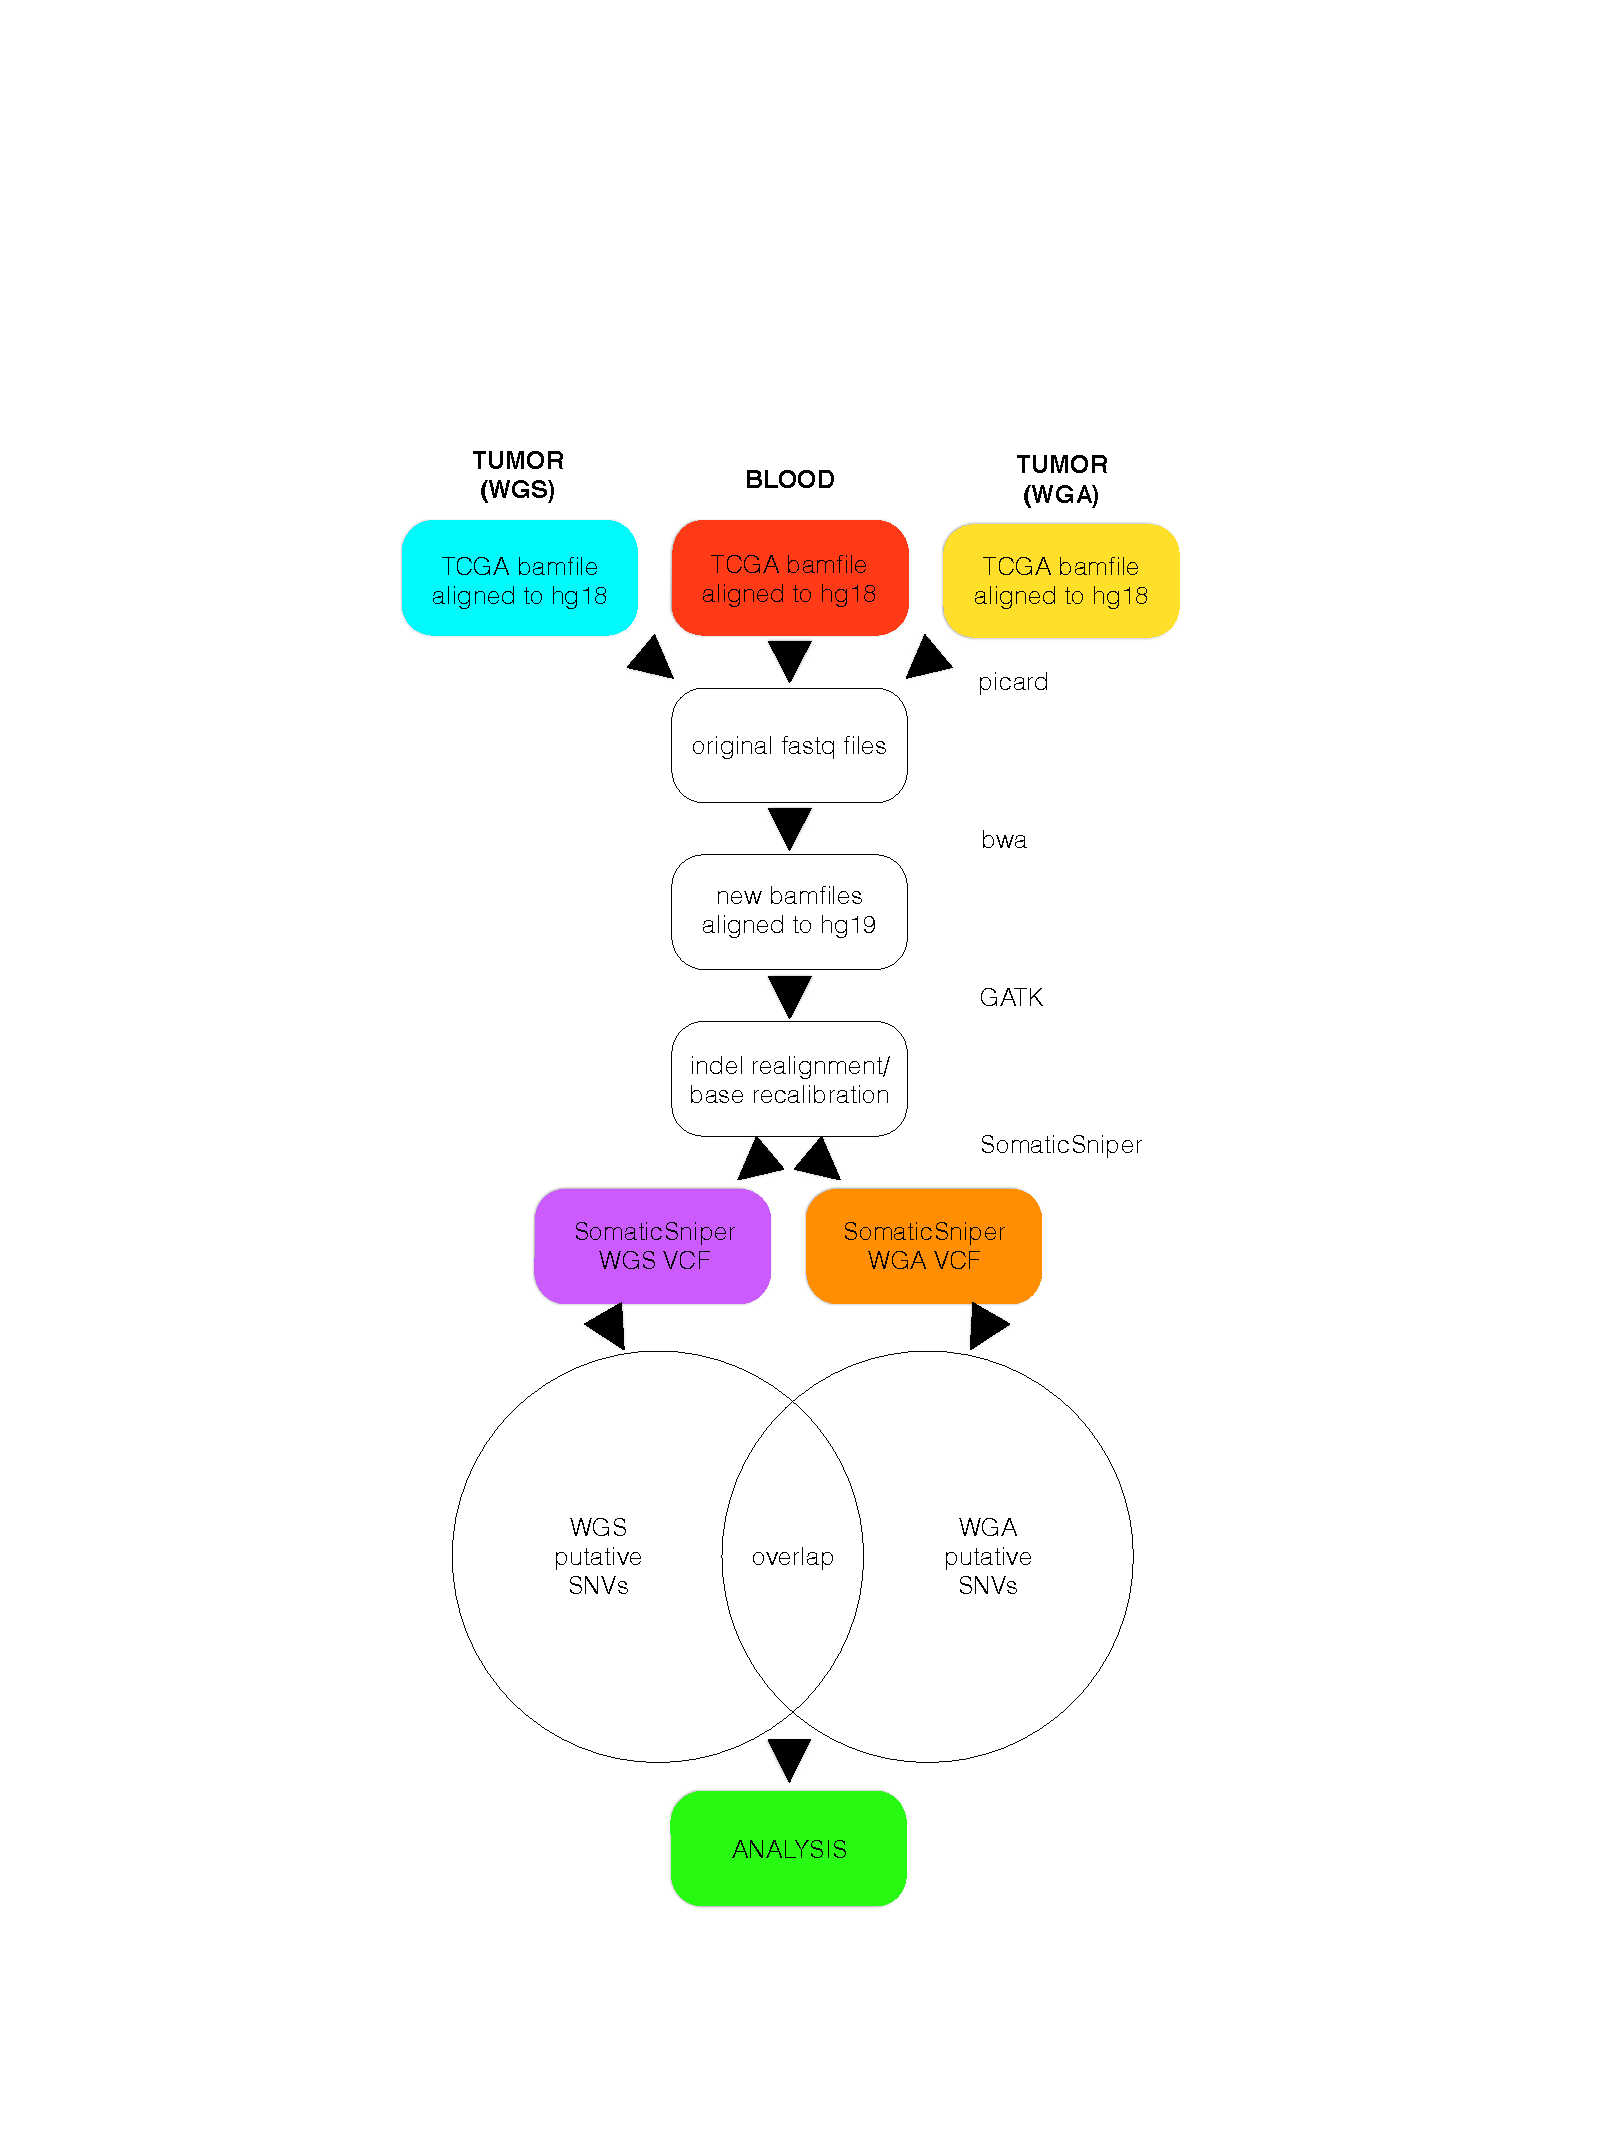
\includegraphics[width=5in]{pipeline.pdf} 
%}
\caption{\textbf{Data processing pipeline.} For each of 55 patients, we began with a C484 tumor BAM file (WGS), a C282 tumor BAM file (WGA), and a normal BAM file, all aligned to hg18. For each BAM file, we used picard to regenerate fastq files, bwa to realign the fastq files to hg19, and GATK to recalibrate bases and indels. We used SomaticSniper to call somatic mutations (differences between the tumor and normal sequences) for each replicate. When we had a VCF for each replicate, we calculated the overlap between the two lists as the number of individual mutations which appeared in both replicates.}
\label{fig:pipeline}
\end{figure}

%% Figure 2
\begin{figure}
%\centerline{
%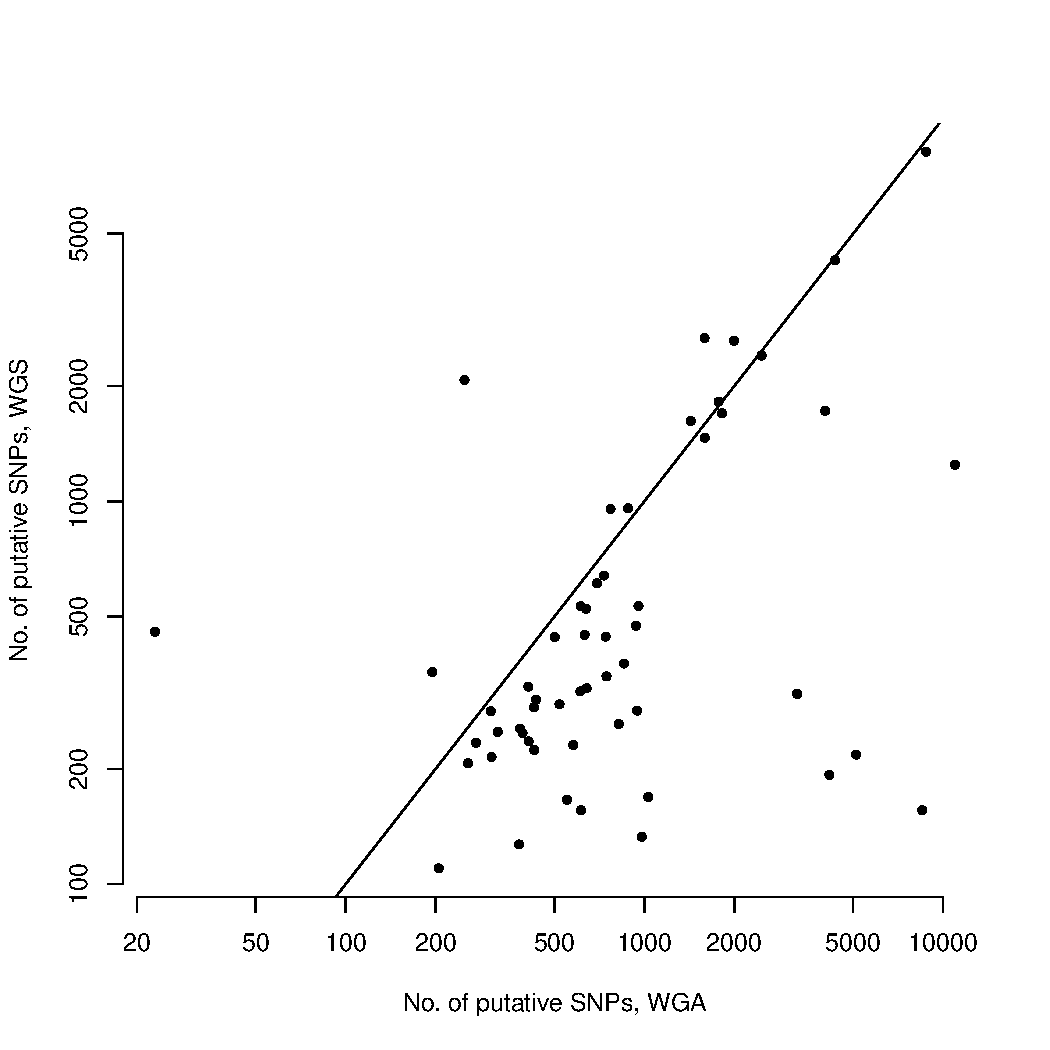
\includegraphics[width=5in]{C282_v_C484.pdf} 
%}
\caption{\textbf{Number of putative SNVs in WGS v.\ WGA, as called by SomaticSniper before filtering.} Each point represents data for a single patient. The line is $y=x$, so points falling below the line agree with the hypothesis that an additional amplification step produces more sequencing errors in a sample. The number of mutations found in one replicate correlates with the number of mutations found in the other replicate (Pearson $r=0.51$, $df = 53$, $P = 8.35\times 10^{-5}$).}
\label{fig:C282_v_C484}
\end{figure}

%% Figure 3
\begin{figure}
%\centerline{
%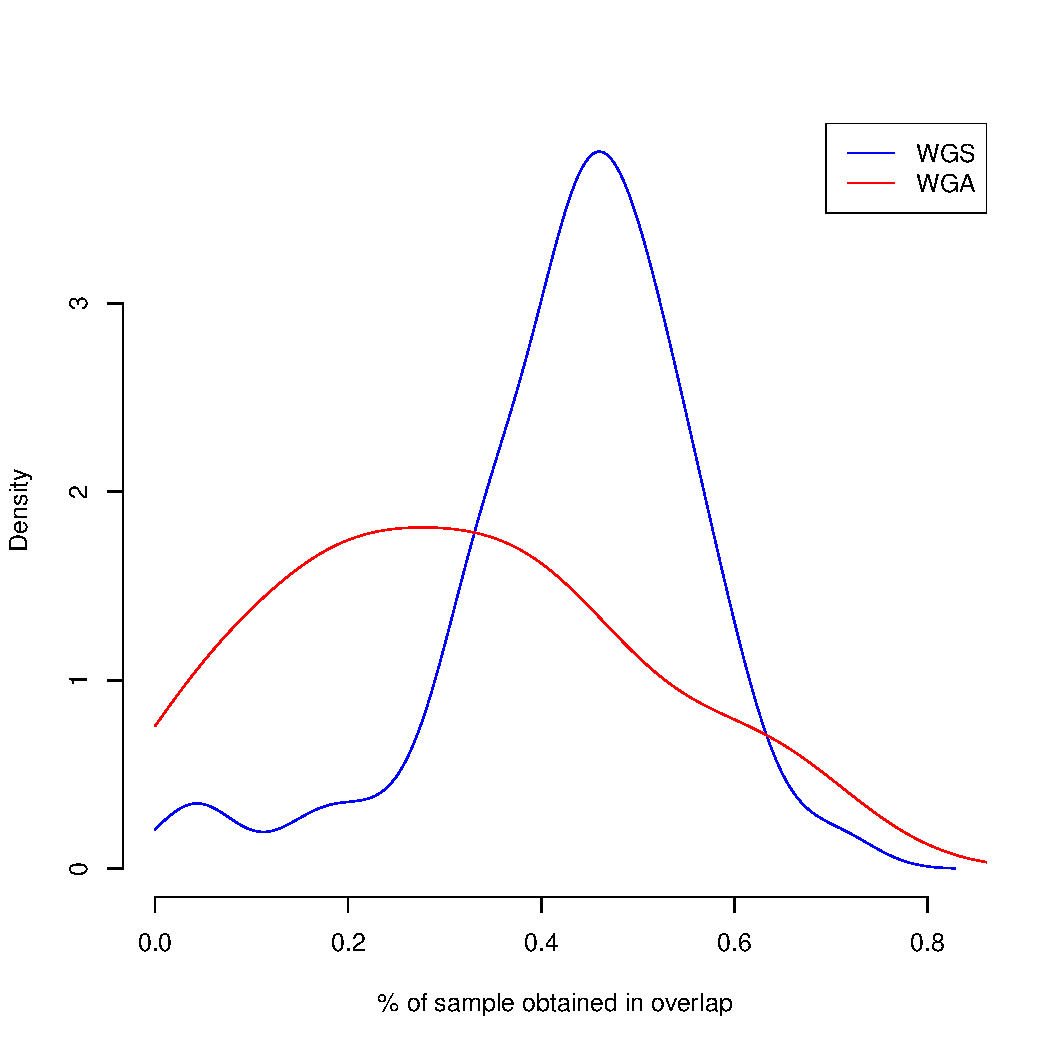
\includegraphics[width=5in]{unfiltered_overlap_WGS_WGA_together_densities.pdf} 
%}
\caption{\textbf{Density of percentage overlap between WGS and WGA samples.} Density of the percentage of each WGS (blue) and WGA (red) sample that is present in the overlap between replicates for each patient. The WGS distribution is higher and narrower, showing that the WGS samples overall have a higher percentage overlap than the WGA samples, and less range in this parameter. }
\label{fig:unfiltered_overlap}
\end{figure}

%% Figure 4
\begin{figure}
%\centerline{
%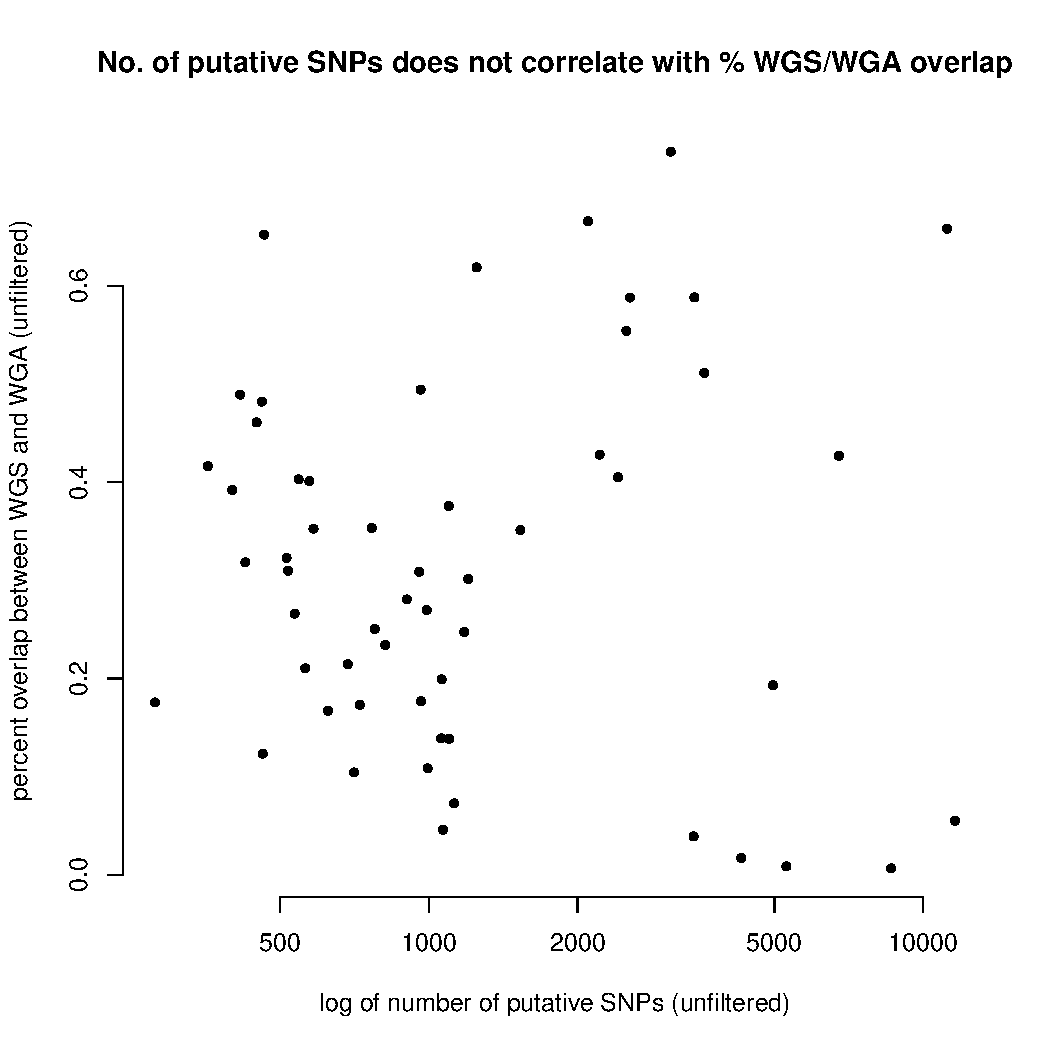
\includegraphics[width=5in]{unfiltered_total_muts_v_percent_overlap.pdf} 
%}
\caption{\textbf{Percent of overlap versus (log) number of putative SNVs per sample.} The percentage of a given WGS sample that is in the overlap between replicates is not correlated to the number of mutations in that sample (Pearson $r=-0.04$, $df=53$, $P=0.76$).}
\label{fig:unfiltered_total_muts}
\end{figure}

%% Figure 5
\begin{figure}
%\centerline{
%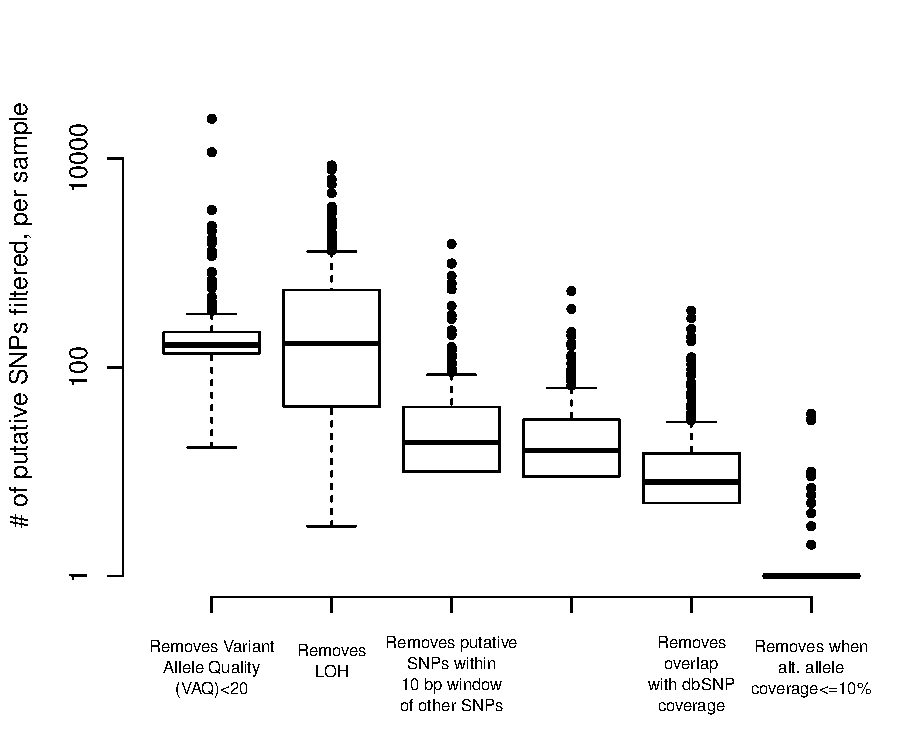
\includegraphics[width=6in]{boxplot_number_filtered.pdf} 
%}
\caption{\textbf{Number of putative SNVs removed by each of six filters.} The $x$-axis gives the name of each filter (detail on Table 1), and the $y$-axis gives, on a log scale, the number of mutations removed by a given filter in a given sample. In all cases, the LOH and VAQ filters removed the majority of the putative SNVs for a given sample.}
\label{fig:boxplot_number_filtered}
\end{figure}

%%Figure 6
\begin{figure}
% 379 samples, 311 patients
%\centerline{
%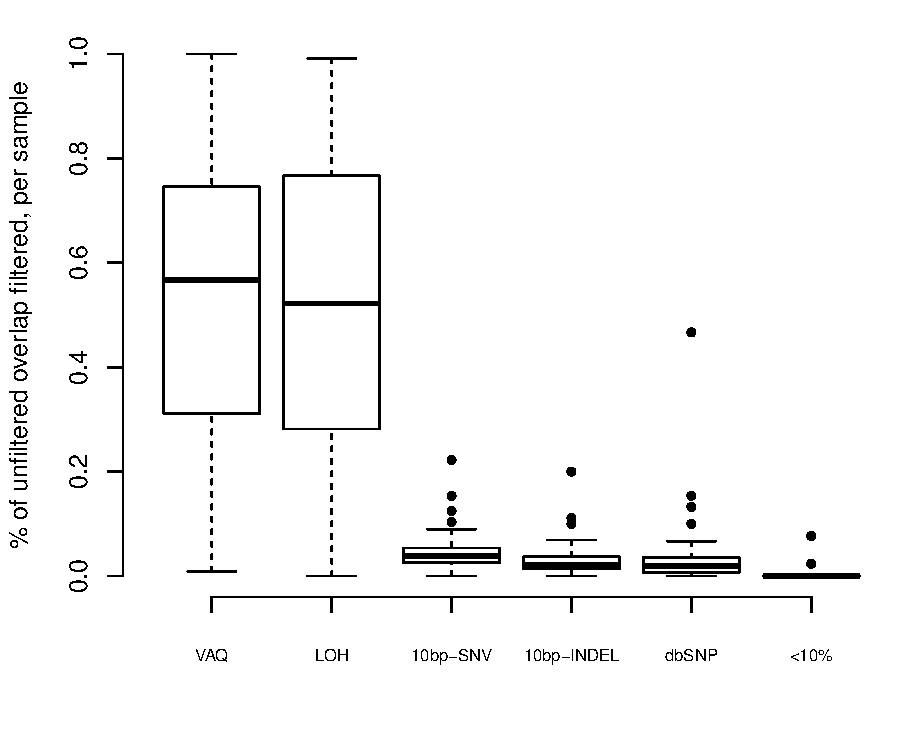
\includegraphics[width=6in]{boxplot_percent_overlap_filtered.pdf} 
%}
\caption{\textbf{Percentage of WGS/WGA overlap removed, by filter.} The $x$-axis gives the names of the filters, and the $y$-axis gives the percentage of the WGS--WGA overlap removed by the filter, per sample. Filters removing LOH and putative SNVs with low VAQ removed a significant percentage of the overlap; nothing else did.}
\label{fig:boxplot_percent_overlap_filtered}
\end{figure}

%%Figure 7
\begin{figure}
%\centerline{
%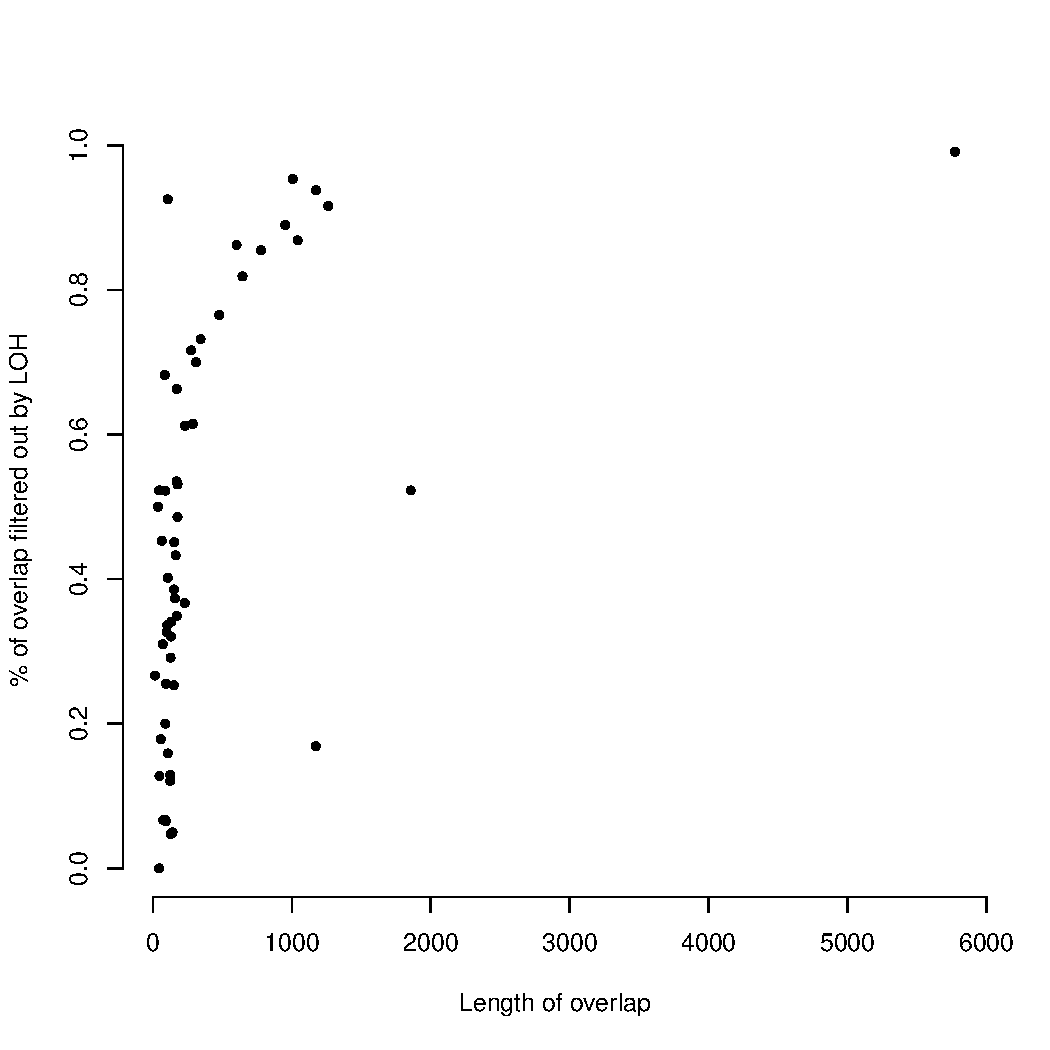
\includegraphics[width=5in]{./LOH_VAQ/LOH_all.pdf} 
%}
\caption{\textbf{Percentage of replicate SNVs filtered out by LOH, as a function of the total number of overlapping SNVs.} As the length of the overlap between WGS and WGA increases ($x$-axis), the percentage of the overlap filtered out by LOH increases. This is the almost (but not quite) perfect inverse of the pattern observed in VAQ mutations (Figure~\ref{fig:VAQ_all}), indicating that these two filters remove almost disjoint sets of putative SNVs.}
\label{fig:LOH_all}
\end{figure}

%%Figure 8
\begin{figure}
%\centerline{
%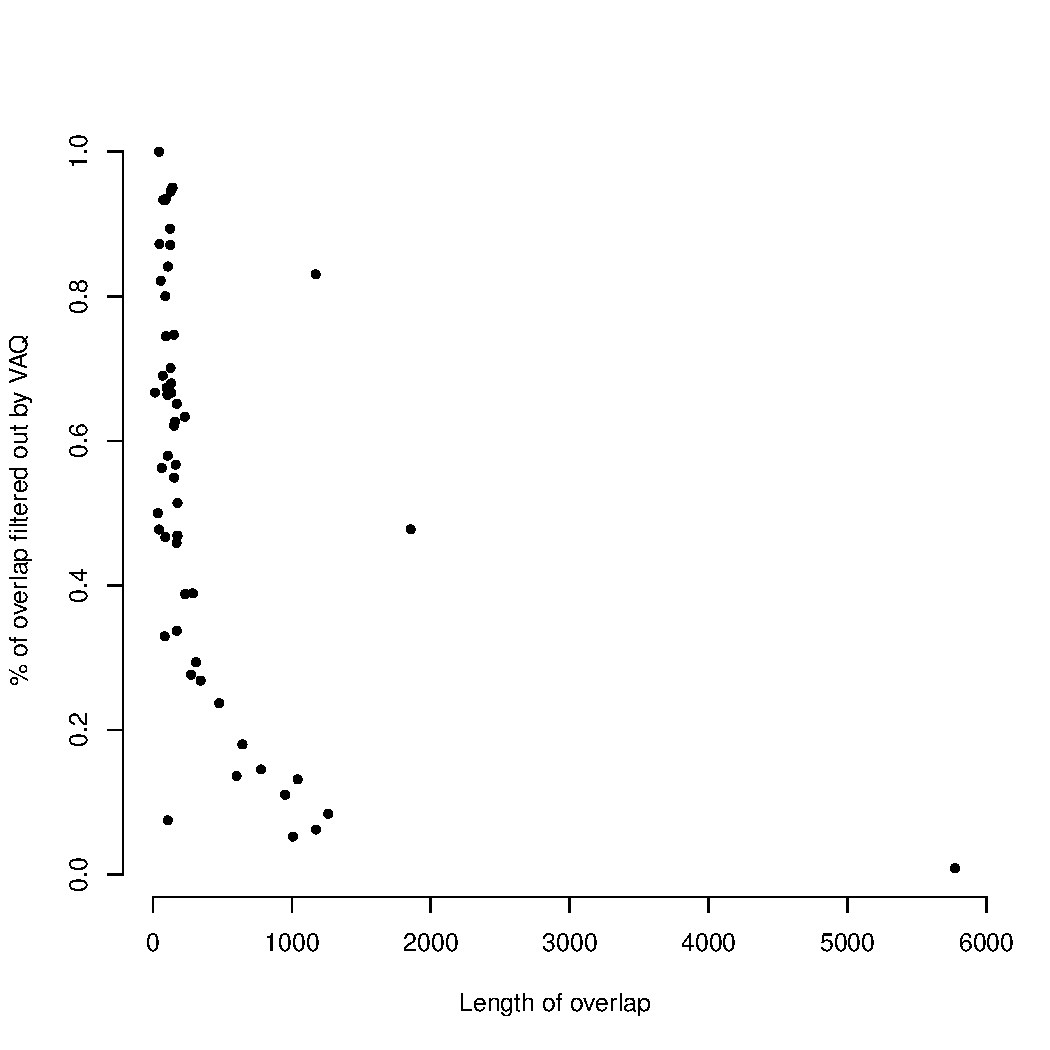
\includegraphics[width=5in]{./LOH_VAQ/VAQ_all.pdf} 
%}
\caption{ \textbf{Percentage of replicate SNVs filtered out by VAQ, as a function of the total number of overlapping SNVs.} As the length of the overlap between WGS and WGA increases ($x$-axis), the percentage of the overlap filtered out by VAQ decreases. This is the almost (but not quite) perfect inverse of the pattern observed in LOH mutations (Figure~\ref{fig:LOH_all}), indicating that these two filters remove almost disjoint sets of putative SNVs.}
\label{fig:VAQ_all}
\end{figure}

\end{document}
